\documentclass[notitlepage]{article}

\usepackage{amsmath}
\usepackage{titling}
\usepackage{graphicx}
\usepackage[margin=1.5in]{geometry}
\usepackage{cite}


\graphicspath{{figures/paper/preliminary/}}

\title{Cognitive Mechanisms for Reinforcement Learning Refinement}

\author{
  Krueger, Paul\\
  \texttt{pmk@berkeley.edu,\ \#26969749}
  \and
  Daniels, Dylan\\
  \texttt{dylandaniels@berkeley.edu,\ \#29655144}
}
\date{\today}

\begin{document}

\maketitle

\begin{abstract}
blah blah blah we need to put stuff here.
\end{abstract}

\section*{Introduction}

\section*{Methods}

To explore theories about reinforcement learning in cognition, we constructed a simple two-dimensional maze game whereby an agent was tasked with learning how to reach a terminal goal state from a start state. The terminal goal state confers the agent a reward of 1 point, and resets the agent's location to the starting point (Figure something of maze). We study two different mazes: a \textit{sparse} maze and a \textit{dense} maze. The sparse maze is easier for the agent to solve, but it is also easier for the agent to get stuck in a suboptimal path. The dense maze, on the other hand, has only one clear path to the solution; as a result, we expect heuristic-based pseudorewards to often fail to find the optimal path.

All of our methods are based on a common model-free reinforcement learning paradigm known as Q-learning~\cite{sutton1998reinforcement}, which learns an optimal policy $\pi^*$ over time. Let $\mathcal{S}$ be the set of states and let $\mathcal{A}$ be the set of actions. For each $(s,a) \in \mathcal{S} \times \mathcal{A}$, a value $Q(s,a)$ is learned via the following algorithm. Initially all $Q(s,a)$ are zero. At each state $s$, with probability $1 - \epsilon$, the agent chooses the action $a \in \mathcal{A}$ with the highest value $Q(s,a)$. With probability $\epsilon$ it chooses an action uniformly at random ($\epsilon$ is a hyperparameter that calibrates the explore-exploit tradeoff). Then, after completing the selected action $a$, the agent moves to $s'$ and updates $Q$ by

\begin{equation}
Q(s,a) \leftarrow Q(s,a) + \alpha (R_(s, s') + \gamma \max_{a'} Q(s', a') - Q(s,a))
\label{eq:q-learn}
\end{equation}

where $\alpha$ is the learning rate, $R_(s, s')$ is the reward received at state $s'$, and $\gamma$ is the discount factor. Q-learning will converge with probability one to the optimal policy. 

\subsection*{DYNA Planning}

Using the DYNA framework described in~\cite{sutton1998reinforcement}, we can improve upon the naive Q-learning algorithm by recalling a random set of past moves after each step. From a cognitive science perspective, this type of optimization is interesting because it is as if we are replaying past memories. In other words, is it cognitively advantageous to think about past experiences, and as a result, learn more from them? 

Planning is implemented by re-updating $p$ Q-values randomly at the end of each step using Equation~\ref{eq:q-learn}. Only the most recent action for each state is updated, so DYNA planning favors recency.

\subsection*{Pseudorewards}

Pseudorewards are an intelligible way of conferring extra information to an agent about the reward landscape. Essentially, a small reward is given to the Q-learner whenever they take an action that helps the agent move towards the goal. Pseudorewards are defined by \textit{shaping functions} $F$. Instead of the agent receiving actual reward $R(s, s')$ when moving from state $s \rightarrow s'$, the agent receives an augmented reward $R'(s, s')$ where
\begin{equation}
R'(s, s') = R(s, s') + F(s, s')
\end{equation} 

 In~\cite{ng1999policy}, conditions for which the optimal policy $\pi^*$ remains invariant under a \textit{shaping function} are developed. If the shaping function does not possess this invariance policy, it is possible that Q-learning will converge to a suboptimal solution. The simplest example of an invariant shaping function uses the difference in optimal values between the agent's current state and next state:
\begin{equation}
F(s, s') = \gamma V_{\pi^*}(s') - V_{\pi^*}(s) 
\end{equation}
\begin{equation}
V_{\pi^*}(s) =  \max_{a} R(s, s') + \gamma V_{\pi^*}(s')
\end{equation}
We call this method the \textit{optimal policy pseudoreward}--it encourages the agent to always move down the optimal path from its current state. If $\epsilon = 0$, the agent would move directly to the goal along the shortest path.

While the \textit{optimal policy pseudoreward} performs well in practice, it's a bit unrealistic for the agent to have such a complete information set in most applications. To compute the optimal policy, the agent must solve a linear program and have full information about states, actions, transitions, and goal states. A more realistic set of pseudorewards can be derived by approximating the distance to the goal. Intuitively, this corresponds to the agent generally knowing which direction to move in. We call this the \textit{Manhattan pseudoreward}.

\begin{figure}[ht]
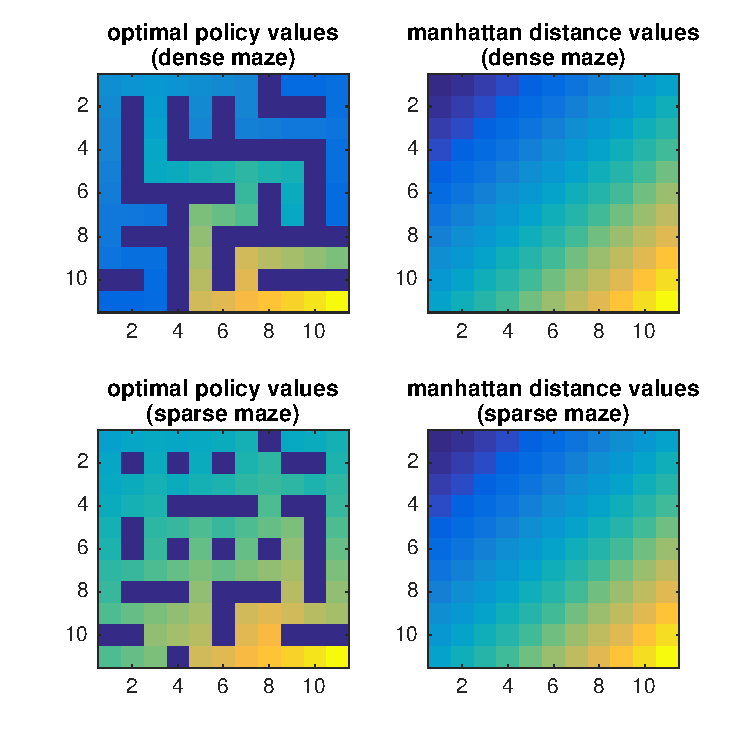
\includegraphics[width=\textwidth]{value_landscapes}
\caption{The landscape of pseudorewards for each maze and each pseudoreward type. Pseudorewards are concocted so that the agent is incentivized to move towards the goal state in the lower rightmost square.}
\label{fig:value-landscapes}
\end{figure}

For our maze environment, we use a modified Manhattan distance metric to implement distance-based pseudorewards. We define the Manhattan distance metric as $\Phi(s) = \gamma^T$, where $T$ is the Manhattan distance, to form the pseudoreward
\begin{equation}
F(s, s') = \gamma \Phi(s') - \Phi(s)
\end{equation} 
which fulfills the conditions in~\cite{ng1999policy} to be an invariant reward transformation. A comparison the pseudoreward landscape for each of the types of the pseudorewards considered is shown in Figure~\ref{fig:value-landscapes}.

In addition, we also test the sensitivity of both pseudoreward methods to additive white noise. For each pseudoreward $F(s, s')$ conferred, let
\begin{equation}
\tilde{F}(s, s') = F(s, s') + e_t
\end{equation} 

\noindent where $e_t \sim N(0, \sigma^2)$. The larger the value of $\sigma$, the more noisy the pseudoreward $\tilde{F}$. In general pseudorewards $\tilde{F}$ will not lead to invariant policies.

\section*{Experiments}

\begin{figure}[ht]
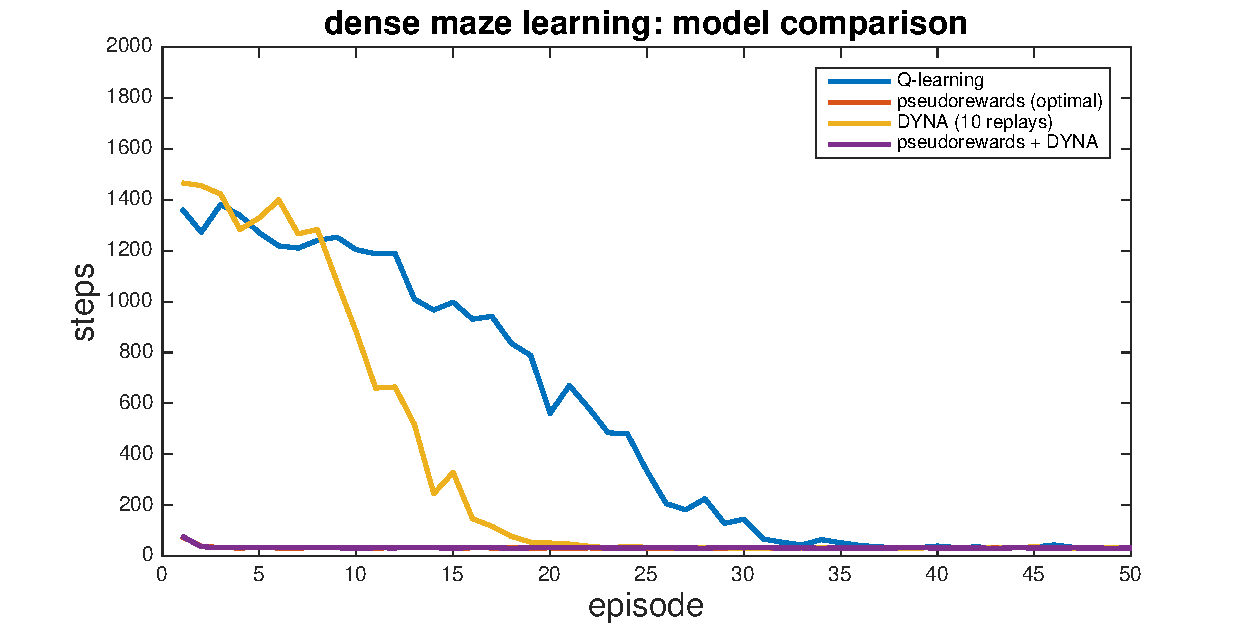
\includegraphics[width=\textwidth]{modelCompare_dense}
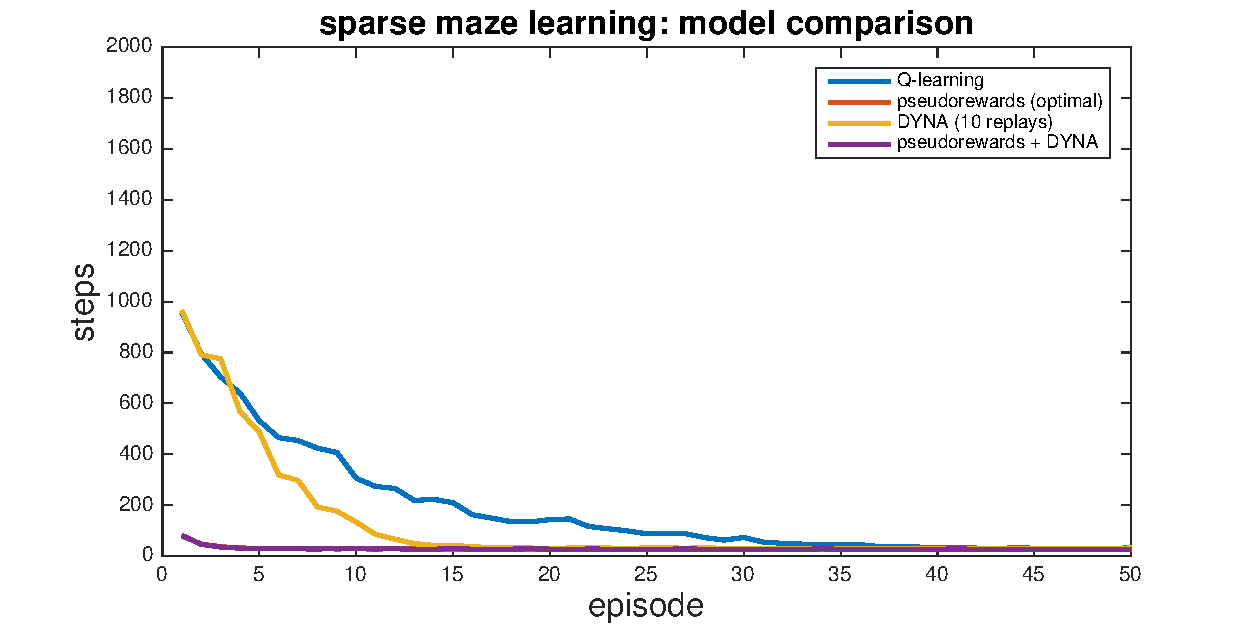
\includegraphics[width=\textwidth]{modelCompare_sparse}
\caption{The mean number of steps taken for each episode are plotted above for Q-learning and 3 variants. The mean is taken over 100 simulations of 50 episodes.}
\label{fig:model-compare}
\end{figure}

To analyze the performance of our agent in each of our two maze environments: \textit{sparse} and \textit{dense}, we ran 100 simulations of reinforcement learning for each condition. In each simulation, we allowed the agent to learn for 50 episodes; the agent automatically advanced to the next episode without reward if a maximum of 2000 steps was reached. For all of our experiments, we set the learning rate $\alpha = 0.1$, the exploratory probability $\epsilon = 0.25$, and the discount factor $\gamma = 0.95$. 

As a first pass, we compare the DYNA architecture with 10 replays with the optimal policy pseudoreward architecture (Figure~\ref{fig:model-compare}). All methods converge to the optimal number of steps: 20 for sparse, 24 for dense. DYNA converges more quickly than regular Q-learning, validating the hypothesis that replaying memories speeds up the learning process. We also see that the optimal policy pseudoreward converges nearly instantly to the optimal value, which is expected because the agent is incentivized to follow the optimal path from the start. When the optimal policy pseudoreward is combined with DYNA for replaying memories, it converges just as fast. 

Next, in Figure~\ref{fig:dyna-compare} we analyze the performance of DYNA by varying the number of moves replayed at the conclusion of each episode. As the number of replays increases, the convergence rate of Q learning increases. It is interesting to note that as a function of episodes, the dense maze appears to have a concave shape while the sparse maze has a convex shape. This means that the majority of learning happens later for the dense maze than for the sparse maze. This is probably due to the fact that it takes longer for the agent to find the optimal path in the dense maze, but once it finds it, learning happens rapidly after. 

\begin{figure}[ht]
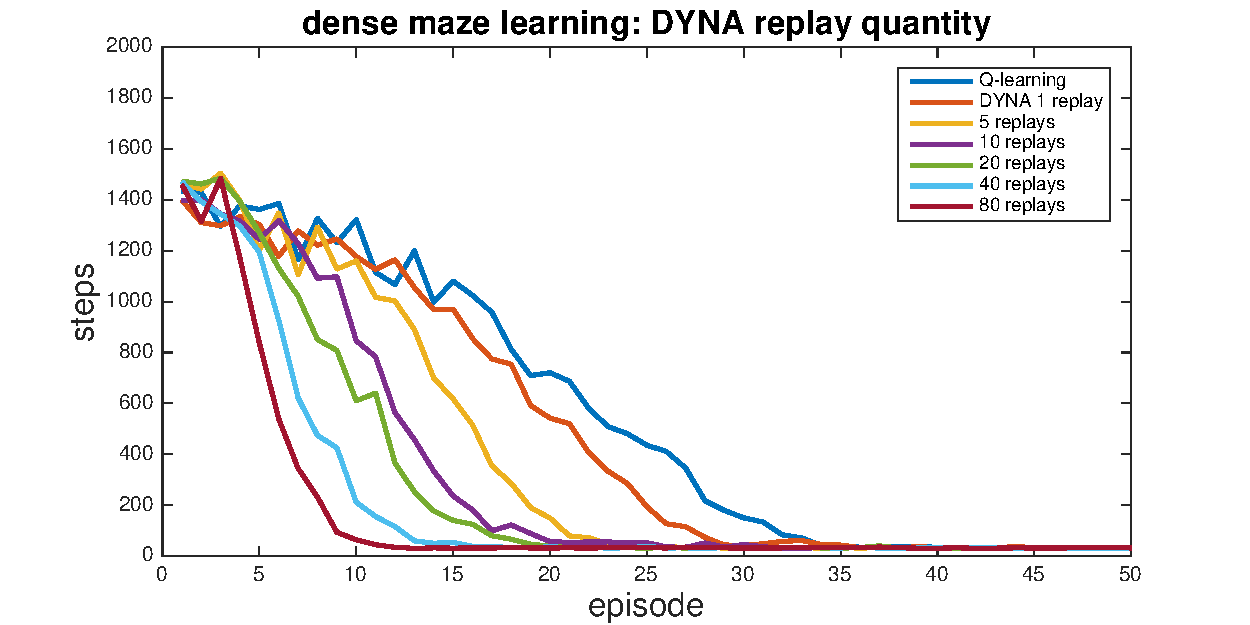
\includegraphics[width=\textwidth]{DYNAcompare_dense}
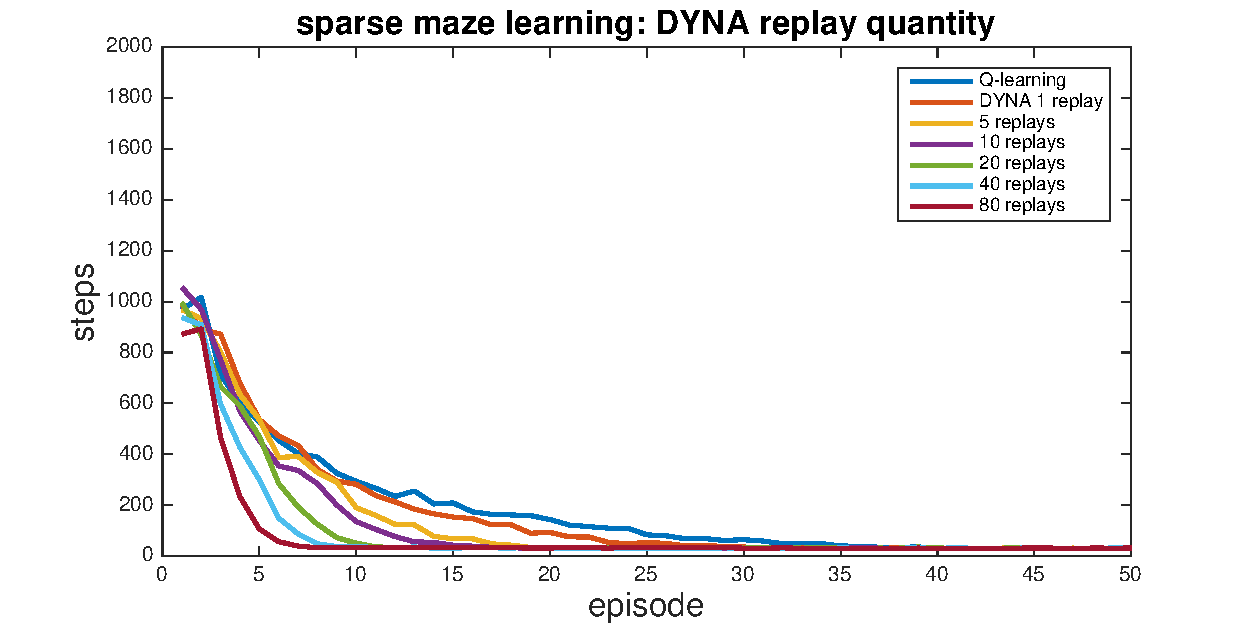
\includegraphics[width=\textwidth]{DYNAcompare_sparse}
\caption{The mean number of steps taken for 100 simulations of DYNA learning. The convergence rate increases with the number of replays.}
\label{fig:dyna-compare}
\end{figure}

We finally compare the performance of our two pseudoreward strategies. As can be seen in Figure {something}, 


\section*{Discussion}

\section*{References}

\bibliography{final_report}{}
\bibliographystyle{apalike}

\end{document}